\chapter{Lab Report}
\section{Week 1}
    This week comprised of performing a Fourier Transform and Inverse Fourier Transform on a .pgm image file. The original image is of a wolf shown in Figure \ref{fig:wolf_image}

    Supporting Java classes were provided, these include Display2dFT.java, DisplayDensity.java, ReadPGM.java and SimpleFT a skeleton program to code in.

    DisplayDensity.java displays a greyscale image from a 2D array, with smaller values dark and larger values white. ReadPGM.java parses the .pgm file for use in the skeleton program and Display2dFT.java allows the Fourier Transform output to be represented graphically, using colour to represent imaginary number components.
    
    \begin{figure}[H]
        \centering
        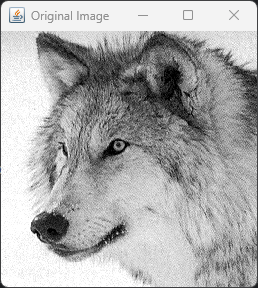
\includegraphics[width=0.49\columnwidth]{Figures/Week 1/W1-Wolf-Original.png}
        \caption{A screenshot of the original wolf image}
        \label{fig:wolf_image}
        
    \end{figure}
    
    \subsection{Discrete Fourier Transform}
    The equation shown in Figure \ref{fig:equation-FT} needs to be implemented to perform a Discrete Fourier Transform, C is an array N, N in size.
    \vspace{15mm}


    \begin{center}
        \begin{equation}
            C_{kl} = 1/N^2 \sum_{m=0}^{N-1} \sum_{n=0}^{N-1}\ X_{mn} . e^{-2\pi i(km+nl)/N}
            \label{fig:equation-FT}
        \end{equation}  
    \end{center}




    
    \begin{figure}[H]
        \centering
        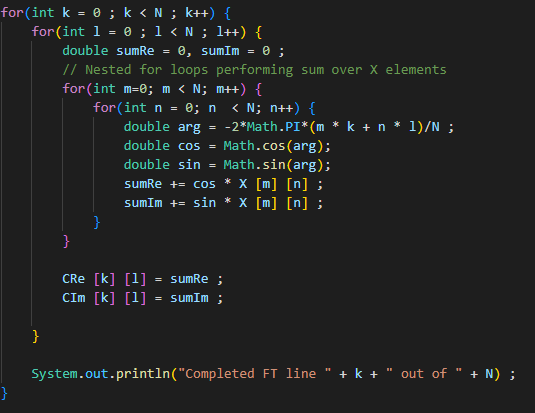
\includegraphics[width=0.49\columnwidth]{Figures/Week 1/W1-SimpleFT-Completed-For-Loop.png}
        \caption{A screenshot of the implementation of the Fourier Transform}
        \label{fig:wolf-FT-code}
    \end{figure}
    
    \begin{figure}[H]
        \centering
        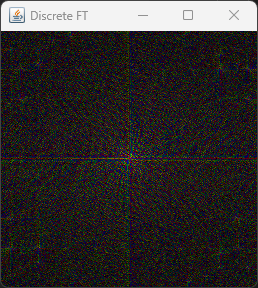
\includegraphics[width=0.49\columnwidth]{Figures/Week 1/W1-FT.png}
        \caption{A screenshot of the Discrete Fourier Transform graphical output}
        \label{fig:wolf-DFT}
    \end{figure}
    
    
    \subsection{Inverse Discrete Fourier Transform}


        \begin{center}
        \begin{equation}
            X_{mn} = \sum_{k=0}^{N-1} \sum_{l=0}^{N-1}\ C_{kl} . e^{2\pi i(km+nl)/N}
            \label{fig:equation-InverseFT}
        \end{equation}  
        \end{center}

        \begin{figure}[H]
            \centering
            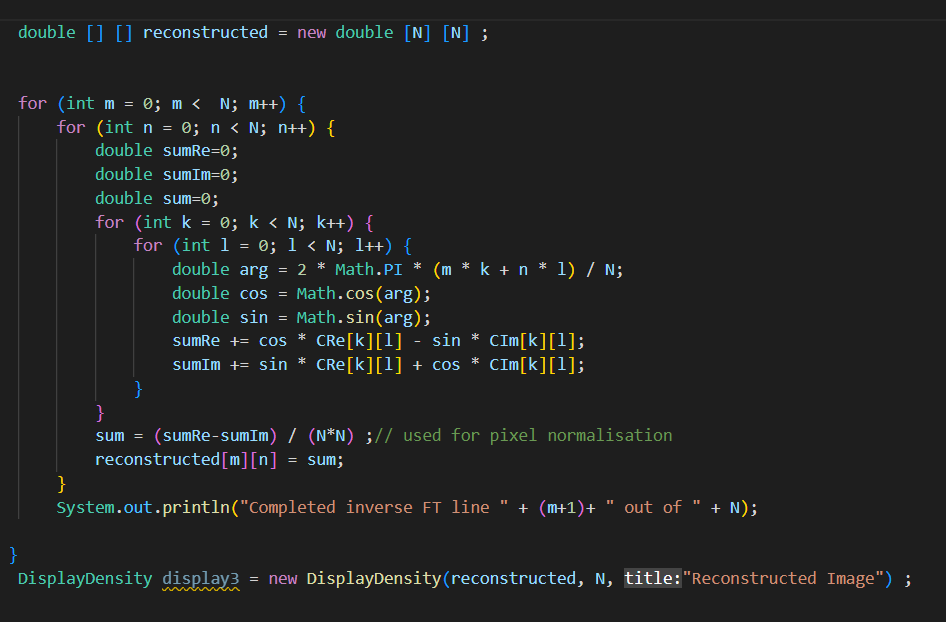
\includegraphics[width=0.49\columnwidth]{Figures/Week 1/W1-SimpleFT-InverseDFT-Implementation.png}
            \caption{A screenshot of the java inverse DFT implementation}
            \label{fig:inverse-DFT-Code}
    \end{figure}
    
        \begin{figure}[H]
            \centering
            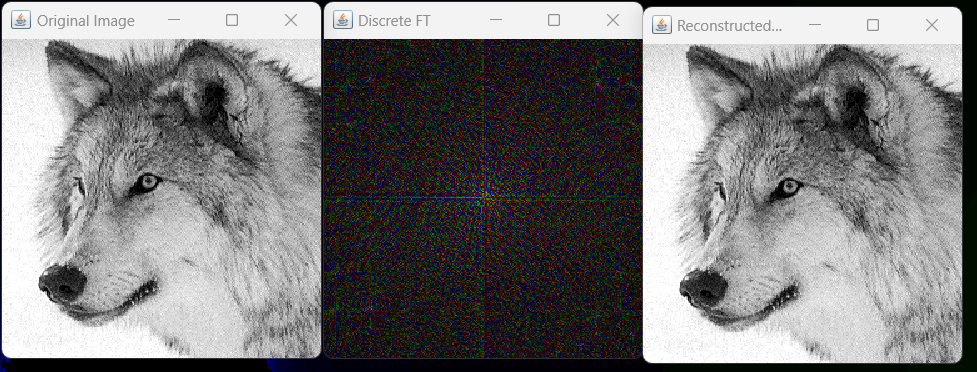
\includegraphics[width=0.49\columnwidth]{Figures/Week 1/W1-SimpleFT-InverseDFT-Graphical-Outputs.png}
            \caption{Graphical output of the program - inverse DFT reconstruction on the right side}
            \label{fig:inverse-DFT-Images-Output}
    \end{figure}
    
        \begin{figure}[H]
            \centering
            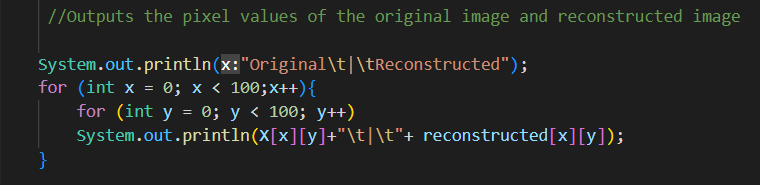
\includegraphics[width=0.49\columnwidth]{Figures/Week 1/W1-SimpleFT-InverseDFT-Test-1.0-code.png}
            \caption{A screenshot of the testing code}
            \label{fig:Testing-Code}
    \end{figure}
    
    \begin{figure}[H]
        \centering
        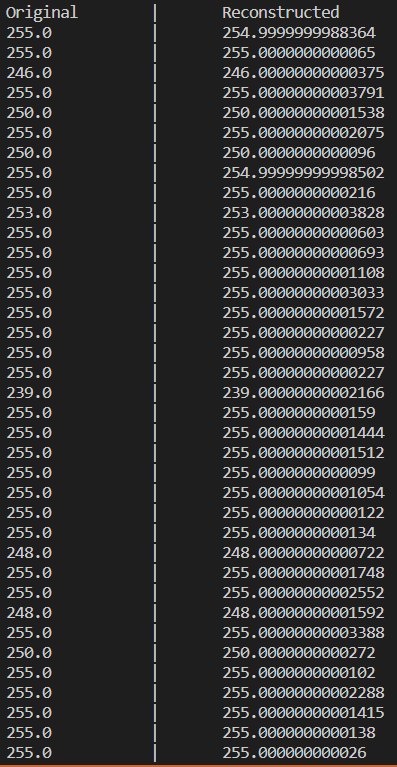
\includegraphics[width=0.49\columnwidth]{Figures/Week 1/W1-SimpleFT-InverseDFT-Test-1.0-Output.png}
        \caption{A screenshot of the testing code output}
        \label{fig:Testing-Code-output}
    \end{figure}
    
    \begin{figure}[H]
        \centering
        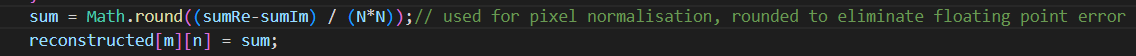
\includegraphics[width=0.49\columnwidth]{Figures/Week 1/W1-SimpleFT-InverseDFT-Floating-Point-Fix.png}
        \caption{A screenshot of code to fix floating point error}
        \label{fig:floating-Point-Fix}
    \end{figure}


    \begin{figure}[H]
        \centering
        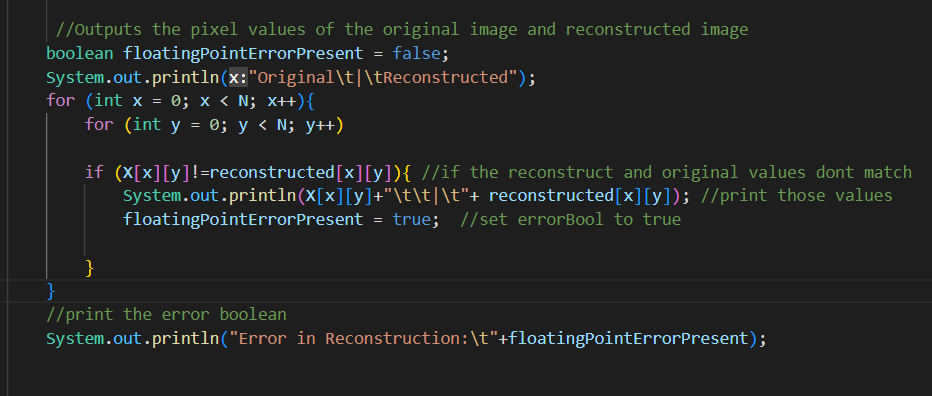
\includegraphics[width=0.49\columnwidth]{Figures/Week 1/W1-SimpleFT-InverseDFT-Test-2.0-code.png}
        \caption{A screenshot of code to test the floating point error fix}
        \label{fig:floating-Point-Fixed-test}
    \end{figure}

    \begin{figure}[H]
        \centering
        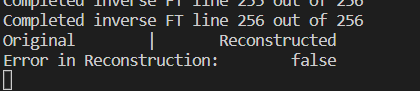
\includegraphics[width=0.49\columnwidth]{Figures/Week 1/W1-SimpleFT-InverseDFT-Test-2.0-CLI-Output.png}
        \caption{A screenshot of console output showing floating point error test has passed}
        \label{fig:floating-Point-Fixed-CLI-Output}
    \end{figure}
    
    \begin{figure}[H]
        \centering
        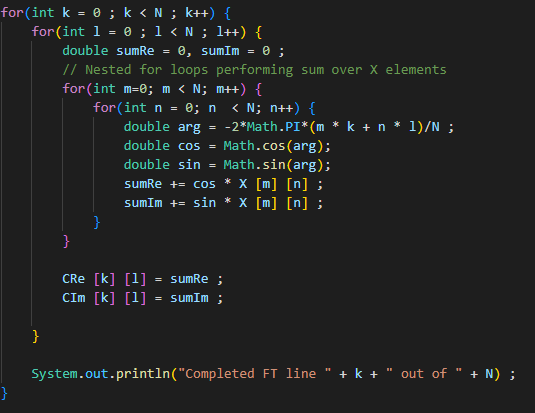
\includegraphics[width=0.49\columnwidth]{Figures/Week 1/W1-SimpleFT-Completed-For-Loop.png}
        \caption{A screenshot of graphical image reconstruction floating point error fix}
        \label{fig:floating-Point-Fixed-Graphical-Output}
    \end{figure}

    
\subsection{}

\section{Week 2}
\section{Week 3}
\section{Week 4}
\section{Week 5}
\section{Week 6}
\section{Week 7}
\section{Week 8}
\section{Week 9}
\section{Week 10}
\section{Week 11}
